\chapter{Metodologia}

Grande parte desta dissertação passa então pela conceção e implementação de um sistema de software, e devido a tal, serão utilizadas práticas de desenvolvimento comprovadas na indústria e que se adequem à natureza do projeto. Nesta capítulo iremos então detalhar as abordagens que irão ser adotadas, assim como as suas vantagens relativas.

\section{Desenvolvimento Iterativo e Incremental}

Esta prática consiste numa combinação de práticas incrementais e iterativas, onde essencialmente um produto de software é separado em componentes, sendo que cada um destes componentes é iterativamente implementado. Essencialmente, esta metodologia de desenvolvimento irá ter os seguintes passos, para a elaboração de cada componente:
\begin{itemize}
    \item Requisitos - definição dos requisitos do sistema
    \item Design/Arquitetura - desenho da arquitetura do sistema
    \item Implementação - implementação dos elementos definidos na arquitetura
    \item Testes - testes unitários e de integração
    \item Avaliação - avaliação do sistema dum ponto de vista funcional e técnico
\end{itemize}

Durante a idealização da arquitetura, o sistema irá ser dividido em pequenos componentes ou sistemas que resultam no projeto final, sendo que cada um sistema irá ser implementado um de cada vez, seguindo esta metodologia. Na essência, esta metodologia é uma combinação da metodologia \textit{Waterfall} e incremental, desenvolvendo pequenas partes do sistema de cada vez.

\section{Desenvolvimento Orientado a Modelos}

Ideal para sistemas de grande complexidade, durante o desenvolvimento dos componentes de software deste projeto irão ser utilizados diagramas para descrever o comportamento do sistema a um nível de abstração elevado. Utilizando modelos de domínio e diagramas de classe, entre outros, será possível descrever a um alto nível de abstração, a estrutura e o comportamento do sistema de software antes da sua implementação.

Esta metodologia tem grandes vantagens, sendo uma delas a facilitação do trabalho em equipa e a colaboração com outros, uma vez que é mais fácil explicar conceitos através de um diagrama em vez de um excerto de código. Além disso, dado que os diagramas não estão necessariamente ligados a uma dada tecnologia ou linguagem de programação, teremos uma grande vantagem na altura de migrar o sistema para outra tecnologia, caso seja necessário. Além disso, existem aplicações no mercado, capazes de transformar modelos em código, reduzindo o tempo de implementação necessário.

Neste preciso caso, será utilizado UML para desenhar os diagramas, uma linguagem de modelação bastante utilizada na indústria, possuindo várias ferramentas capazes de transformar diagramas em código.

\section{Análise Estática de Código}

Sistemas de software de  grande dimensão devem seguir os mesmos standards sintáticos e arquiteturais em toda o código. Para efetuar esta verificação, serão utilizadas ferramentas de análise de código, que permitirão detetar \textit{code smells} e más práticas arquiteturais para prevenir \textit{bugs} e falhas de segurança. Também ajudam a manter o estilo do código uniforme, para melhorar a sua legibilidade e compreensibilidade.

\section{Integração Contínua}

Todos os componentes do sistema irão ser mantidos num sistema de controlo de versões, nomeadamente o \textit{git}, utilizando o serviço de \textit{hosting} do \textit{GitHub}. Utilizando este serviço, é possível efetuar várias integrações com outras ferramentas de \textit{testing} e \textit{deployment} que nos permitem seguir esta metodologia de \textit{continuous integration}, onde se testa e coloca-se uma aplicação pronta para ambientes de produção continuamente, sem a interação manual dos programadores.

Utilizando estes recursos é possível testar a última versão do código assim que ele é disponibilizado no repositório \textit{GitHub}. Para isto recorremos ao \textit{Travis}, que possui uma integração com dedicada com o \textit{GitHub}, possibilitando esta ''integração contínua''. Além dos testes, também são executadas nesta fase as ferramentas de análise de código, retornando uma \textit{build} errónea caso elas detetem problemas.

\begin{figure}[H]
  \centering
        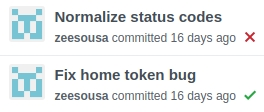
\includegraphics[scale=0.65]{img/github.jpg}
  \caption{Integração Travis \& GitHub}
\end{figure}

Na Figura 7, o \textit{commit} ''Fix home token bug'' passou os testes definidos enquanto que o último \textit{commit} ''Normalize status codes'' falhou os testes.

Quanto a metodologia dos testes não foi seguida nenhuma em específico, apenas foi feito um esforço para se ter o maior número de linhas de código e funcionalidades cobertas pelos mesmos.

Em todos os repositórios é possível obter um \textit{coverage report}, que relata a cobertura dos testes sobre as aplicações. Para isto recorreu-se ao serviço \textit{codecov}, que gera estes relatórios automaticamente a partir do \textit{Travis}.

\begin{figure}[H]
  \centering
        
\includegraphics[scale=0.65]{img/github-badges.jpg}
  \caption{Integração Travis \& GitHub}
\end{figure}

Para comprovar isto, podemos ver, na Figura 8, dois crachás gerados pelo \textit{codecov} e pelo \textit{Travis} respetivamente, que denotam a cobertura do código no que toca a testes, assim como o estado dos testes feitos à ultima \textit{build}.

Os componentes do sistema que necessitarem de um sistema de \textit{hosting} irão recorrer ao \textit{Heroku}, uma \textit{platform as a service}, que permite correr qualquer tipo de serviço web sem custos. A única limitação consiste no adormecimento dos serviços, ou seja, todos os serviços grátis ''adormecem'' ao fim de 30 minutos sem receberem qualquer tráfego.

O \textit{Heroku} é semelhante ao \textit{Travis} na medida em que sempre que deteta novas alterações no \textit{GitHub}, ele tenta efetuar o \textit{deploy} dessa nova versão. Neste caso, como também temos o \textit{Travis} no nosso \textit{workflow}, o \textit{Heroku} aguarda que os testes passem antes de dar \textit{deploy} ao código. Assim, asseguramos que a versão do sistema ativa é estável.

Mesmo assim, nem sempre é possível testar uma aplicação com mecanismos automáticos, devendo sempre ser feitos testes mais extensos recorrendo a utilizadores reais ou à operação manual da aplicação. Para resolver isto, o \textit{Heroku} disponibiliza um mecanismo de \textit{pipelines} avançado, podendo ter a aplicação disponível em vários ambientes. No nosso caso, temos o ambiente de testes, onde estava sempre a última versão da aplicação, que serve para estes tais testes mais extensos. Depois, temos por fim o ambiente de produção, onde se deve efetuar o \textit{deploy} manual de uma versão, por exemplo, depois de testar extensivamente uma versão que tem estado no ambiente de testes, podemos decidir promover-la ao ambiente de produção.

